\documentclass[电力电子]{subfiles}
\begin{document}
\section{简答题}
\begin{ti}[5 分]
	维持晶闸管导通的条件是什么?怎样才能使晶闸管由导通变为关断?
\end{ti}

\begin{ti}[5 分]
	试说明 PWM 控制的基本原理。
\end{ti}

\begin{ti}[5 分]
	简述升压斩波电路的工作原理。
\end{ti}

\begin{ti}[5 分]
	无源逆变电路和有源逆变电路有何不同?
\end{ti}

\begin{ti}[10 分]
	画出降压斩波电路原理图并简述其工作原理。
\end{ti}

\begin{ti}[10 分]
	画出单相半桥电压型逆变电路原理图,并简述其工作原理。
\end{ti}

\begin{ti}[10 分]
	画出单相全桥电压型逆变电路原理图,并简述其工作原理。
\end{ti}

\begin{ti}[5 分]
	单极性和双极性 PWM 调制有什么区别?
\end{ti}

\begin{ti}[5 分]
	什么是异步调制?什么是同步调制?
\end{ti}

\begin{ti}[5 分]
	常用电力电子器件有哪些?
\end{ti}

\begin{ti}[5 分]
	什么叫交—交变频电路?
\end{ti}

\begin{ti}[5 分]
	常用电力电子器件有哪些?
\end{ti}

\begin{ti}[5 分]
	电力电子器件有哪四种工作状态?
\end{ti}

\begin{ti}[5 分]
	单相交流调压电路,控制角 $\alpha$ 的最大移相范围是多少?
\end{ti}

\begin{ti}[5 分]
	维持晶闸管导通的条件是什么?怎样才能使晶闸管由导通变为关断?
\end{ti}

\begin{ti}[5 分]
	什么叫有源逆变?什么叫无源逆变?
\end{ti}

\begin{ti}[12 分]
	画出降压斩波电路的原理图和输出电压电流波形图(电流连续),并分析其工作原理。
\end{ti}

\begin{ti}[12 分]
	画出单相全桥逆变电路的原理图和采用移相调压方式时的控制信号波形图、输出电压波形图,并分析其工作原理。
\end{ti}

\begin{ti}[4 分]
	什么叫交—交变频电路?
\end{ti}

\begin{ti}[4 分]
	常用电力电子器件有哪些?
\end{ti}

\begin{ti}[4 分]
	无源逆变电路和有源逆变电路有何不同?
\end{ti}

\begin{ti}[15 分]
	画出升压斩波电路的原理图和输出电压电流波形图(电流连续),并分析其工作原理。
\end{ti}

\begin{ti}[15 分]
	画出单相半桥逆变电路的原理图和输出电压电流波形图,并分析其工作原理。
\end{ti}

\begin{ti}[4 分]
	维持晶闸管导通的条件是什么?怎样才能使晶闸管由导通变为关断?
\end{ti}

\begin{ti}[4 分]
	晶闸管触发电路的要求?
\end{ti}

\begin{ti}[4 分]
	无源逆变电路和有源逆变电路有何不同?
\end{ti}

\begin{ti}[15 分]
	画出升降压斩波电路的原理图和输出电压电流波形图(电流连续),并分析其工作原理。
\end{ti}

\begin{ti}[15 分]
	画出负载换流电路的原理图和输出电压电流波形图,并分析其工作原理。
\end{ti}

\begin{ti}[5 分]
	分别写出降压斩波电路、升压斩波电路和升降压斩波电路的直流输出电压 $U_{\oo}$ 与电源电压 $E$ 的关系式。
\end{ti}

\begin{ti}[5 分]
	有源逆变的条件。
\end{ti}

\begin{ti}[5 分]
	什么是逆变失败?如何防止逆变失败?
\end{ti}

\begin{ti}[5 分]
	交流调压电路和交流调功电路有什么区别?
\end{ti}

\begin{ti}[10 分]
	脉宽可调的斩波电路如图,说明电路中 V\textsubscript{12} 及 $L$、$C$、V\textsubscript{22} 各有什么作用?\V 承受反压的时间由哪些参数决定?
\end{ti}

\begin{ti}[10 分]
	画出负载换流电路的输出电压电流波形图,并分析其工作原理。
\end{ti}

\begin{ti}[4 分]
	使晶闸管导通的条件是什么?
\end{ti}

\begin{ti}[4 分]
	交流调压电路和交流调功电路有什么区别?
\end{ti}

\begin{ti}[4 分]
	换流方式有几种?哪几种?
\end{ti}

\begin{ti}[4 分]
	什么是电压型逆变电路?有什么特点?
\end{ti}

\begin{ti}[4 分]
	有源逆变失败的原因?
\end{ti}

\begin{ti}[10 分]
	分析单相交交变频电路的整流与逆变工作状态。
\end{ti}

\begin{ti}[5 分]
	脉宽可调的斩波电路如图,说明电路中 V\textsubscript{12} 及 $L_{1}$、$C$、V\textsubscript{22} 各有什么作用?\V 承受反压的时间由哪些参数决定?
\end{ti}

\begin{ti}[5 分]
	有源逆变失败的原因?
\end{ti}

\begin{ti}[5 分]
	在三相全控桥式有源逆变电路中,以连接于 A 相的共阴极组晶闸管 V\textsubscript{1} 为例,说明其在一个周期中,导通及关断期两端承受电压波形的规律。
\end{ti}

\begin{ti}[5 分]
	简述晶闸管的正向伏安特性。
\end{ti}

\begin{ti}[10 分]
	高压直流输电系统原理如图所示,若使功率从左向右传输,变流器 \Rmnum{1}、\Rmnum{2} 分别工作于什么状态?控制角 $\alpha$ 如何?输出电压大小、极性如何?
	\begin{center}
		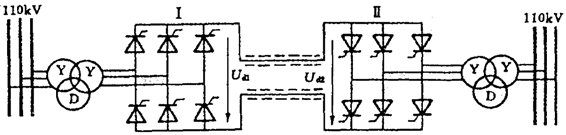
\includegraphics{figure/fig4.png}
	\end{center}
\end{ti}

\begin{ti}[10 分]
	高压直流输电系统原理如图所示,若使功率从左向右传输,变流器 \Rmnum{1}、\Rmnum{2} 分别工作于什么状态?控制角 $\alpha$ 如何?输出电压大小、极性如何?
	\begin{center}
		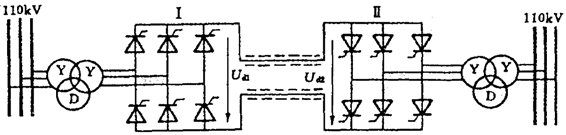
\includegraphics{figure/fig4.png}
	\end{center}
\end{ti}

\begin{ti}[10 分]
	高压直流输电系统原理如图所示,若使功率从左向右传输,变流器 \Rmnum{1}、\Rmnum{2} 分别工作于什么状态?控制角 $\alpha$ 如何?输出电压大小、极性如何?
	\begin{center}
		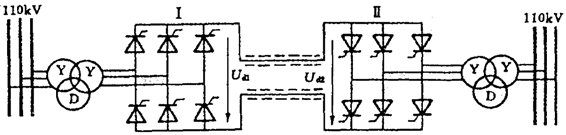
\includegraphics{figure/fig4.png}
	\end{center}
\end{ti}

\begin{ti}[5 分]
	简述交流调功电路的调节方式。
\end{ti}

\begin{ti}[5 分]
	有源逆变的条件。
\end{ti}

\begin{ti}[10 分]
	在三相全控桥式整流电路中,以连接于 A 相的共阴极组晶闸管 V\textsubscript{1} 为例,说明其在一个周期中,导通及关断期两端承受电压波形的规律。
\end{ti}

\begin{ti}[4 分]
	在晶闸管为开关的有源逆变器中两种换流方式是什么?
\end{ti}

\begin{ti}[4 分]
	使晶闸管正常导通的条件是什么?
\end{ti}

\begin{ti}[7 分]
	什么是逆变失败?如何防止逆变失败?
\end{ti}

\begin{ti}[5 分]
	交流调压电路和交流调功电路有什么区别?
\end{ti}

\begin{ti}[5 分]
	有源逆变产生的条件。
\end{ti}

\begin{ti}[5 分]
	维持晶闸管导通的条件是什么?怎样才能使晶闸管由导通变为关断?
\end{ti}

\begin{ti}[5 分]
	维持晶闸管导通的条件是什么?怎样才能使晶闸管由导通变为关断?
\end{ti}

\begin{ti}[5 分]
	无源逆变电路和有源逆变电路有何不同?
\end{ti}

\begin{ti}[5 分]
	试说明 PWM 控制的基本原理。
\end{ti}

\begin{ti}[15 分]
	分析 Cuk 斩波电路的工作原理?
\end{ti}

\begin{ti}[15 分]
	分析下图所示电路的工作原理,并画出 $u_{\oo}$ 的波形图。
	\begin{center}
		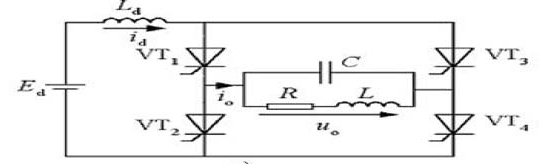
\includegraphics[width=0.5\textwidth]{figure/fig8.png}
	\end{center}
\end{ti}

\begin{ti}[5 分]
	有源逆变失败的原因?
\end{ti}

\begin{ti}[5 分]
	简述晶闸管的正常工作时的特性。
\end{ti}

\begin{ti}[5 分]
	换流方式有几种?哪几种?
\end{ti}

\begin{ti}[5 分]
	什么是逆变失败?
\end{ti}

\begin{ti}[10 分]
	高压直流输电系统原理如图所示,若使功率从左向右传输,变流器 \Rmnum{1}、\Rmnum{2} 分别工作于什么状态?控制角 $\alpha$ 如何?输出电压大小、极性如何?
	\begin{center}
		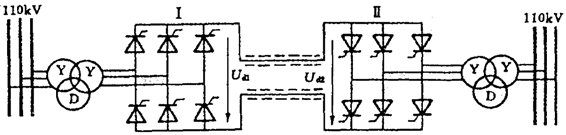
\includegraphics{figure/fig4.png}
	\end{center}
\end{ti}

\begin{ti}[10 分]
	高压直流输电系统原理如图所示,若使功率从左向右传输,变流器 \Rmnum{1}、\Rmnum{2} 分别工作于什么状态?控制角 $\alpha$ 如何?输出电压大小、极性如何?
	\begin{center}
		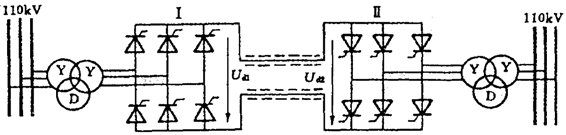
\includegraphics{figure/fig4.png}
	\end{center}
\end{ti}

\begin{ti}[10 分]
	对于桥式可逆斩波电路,若需使电动机工作于正转电动状态,试分析此时电路的工作情况,并绘制相应的电流流通路径图,同时标明电流流向。
\end{ti}

\begin{ti}[5 分]
	交流调压电路的晶闸管控制方式有哪几种?试具体说明。
\end{ti}

\begin{ti}[5 分]
	维持晶闸管导通的条件是什么?怎样才能使晶闸管由导通变为关断?
\end{ti}

\begin{ti}[10 分]
	三相全控桥式整流电路在运行中,当晶闸管触发脉冲丢失或电源缺相,将会出现什么现象,如果是逆变电路又将如何?
\end{ti}

\begin{ti}[10 分]
	高压直流输电系统原理如图所示,若使功率从左向右传输,变流器 \Rmnum{1}、\Rmnum{2} 分别工作于什么状态?控制角 $\alpha$ 如何?输出电压大小、极性如何?
	\begin{center}
		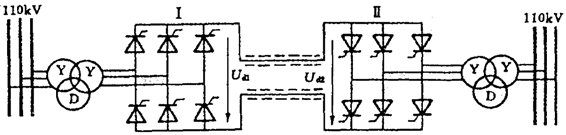
\includegraphics{figure/fig4.png}
	\end{center}
\end{ti}

\begin{ti}[5 分]
	有源逆变产生的条件。
\end{ti}

\begin{ti}[5 分]
	晶闸管的导通条件和关断条件。
\end{ti}

\begin{ti}[5 分]
	什么叫逆变?什么叫有源逆变?什么叫无源逆变?
\end{ti}

\begin{ti}[5 分]
	常用电力电子器件有哪些?
\end{ti}

\begin{ti}[10 分]
	分析下图所示斩波电路的基本工作原理。形状 Q 是可以代替什么元件?
	\begin{center}
		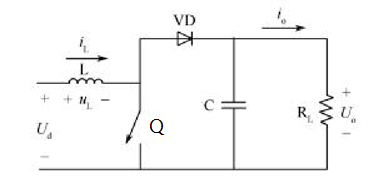
\includegraphics[width=0.5\textwidth]{figure/fig7.png}
	\end{center}
\end{ti}

\begin{ti}[10 分]
	如图为单相桥式 SPWM 逆变器的主电路。试说明单极性控制方式在调制波 $u_{\mathrm{r}}$ 的负半周的控制方法和工作过程。
\end{ti}

\begin{ti}[5 分]
	在单相半波可控整流大电感负载有续流二极管的电路中,晶闸管的控制角 $\alpha$ 的最大移相范围是多少?晶闸管的导通角、续流二极管的导通与 $\alpha$ 关系如何?
\end{ti}

\begin{ti}[5 分]
	交流调压电路和交流调功电路有什么区别?
\end{ti}

\begin{ti}[5 分]
	交交变频电路(采用三相桥式整流电路)的最高输出频率是多少?制约输出频率提高的因素是什么?
\end{ti}

\begin{ti}[5 分]
	电力电子器件有几种工作状态?哪几种?
\end{ti}

\begin{ti}[10 分]
	分析单相交交变频电路的整流与逆变工作状态。
\end{ti}

\begin{ti}[5 分]
	在三相全控桥式有源逆变电路中,以连接于 A 相的共阴极组晶闸管 V\textsubscript{1} 为例,说明其在一个周期中,导通及关断期两端承受电压波形的规律。
\end{ti}

\begin{ti}[5 分]
	有源逆变失败的原因?
\end{ti}

\begin{ti}[5 分]
	维持晶闸管导通的条件是什么?
\end{ti}

\begin{ti}[5 分]
	简述晶闸管的正常工作时的特性。
\end{ti}
\end{document}